\subsection*{Problema 33}
\textbf{Enunciado:} Calcular la integral:
\begin{equation*}
\int \dfrac{x^{-2} \, dx}{(1 + x^4)^{3/4}}
\end{equation*}

\textbf{Solución:} Analizamos el integrando
como un diferencial binomio de la forma:
\begin{equation*}
\int x^{m} (a + b x^n)^{p} \, dx
\end{equation*}
Donde $m = -2$, $n = 4$, $p = -3/4$,
$a = 1$ y $b = 1$. Verificamos el
criterio de Chebyshev:
\begin{align*}
\dfrac{m + 1}{n} + p &= \dfrac{-2 + 1}{4} - \dfrac{3}{4} \\
&= -\dfrac{1}{4} - \dfrac{3}{4} = -1
\end{align*}
Dado que el resultado es un número entero,
utilizamos la sustitución sugerida:
\begin{equation*}
1 + x^{-4} = z^4
\end{equation*}

Diferenciamos ambos lados de la
ecuación para encontrar $dx$:
\begin{align*}
-4x^{-5} \, dx &= 4z^3 \, dz \\
x^{-5} \, dx &= -z^3 \, dz \\
x^{-2} \, dx &= -x^3 z^3 \, dz
\end{align*}

Despejamos $x^4$ de la sustitución
original:
\begin{align*}
x^{-4} &= z^4 - 1 \\
x^4 &= \dfrac{1}{z^4 - 1} \\
x &= (z^4 - 1)^{-1/4}
\end{align*}

Reescribimos el término $(1 + x^4)$
en función de $z$:
\begin{align*}
1 + x^4 &= 1 + \dfrac{1}{z^4 - 1} \\
&= \dfrac{z^4 - 1 + 1}{z^4 - 1} = \dfrac{z^4}{z^4 - 1}
\end{align*}

Sustituimos todo en la integral original:
\begin{align*}
\int &\dfrac{x^{-2} \, dx}{(1 + x^4)^{3/4}} \\
&= \int \dfrac{-x^3 z^3 \, dz}{\left(\dfrac{z^4}{z^4 - 1}\right)^{3/4}}
\end{align*}

Simplificando la expresión algebraica:
\begin{align*}
&= \int \dfrac{-x^3 z^3 (z^4 - 1)^{3/4}}{z^3} \, dz \\
&= -\int x^3 (z^4 - 1)^{3/4} \, dz
\end{align*}

Recordando que $x = (z^4 - 1)^{-1/4}$,
entonces $x^3 = (z^4 - 1)^{-3/4}$:
\begin{align*}
&= -\int (z^4 - 1)^{-3/4} (z^4 - 1)^{3/4} \, dz \\
&= -\int 1 \, dz = -z + C
\end{align*}

Finalmente, regresamos a la variable
original $x$ usando $z = (1 + x^{-4})^{1/4}$:
\begin{equation*}
-\left(1 + x^{-4}\right)^{1/4} + C
\end{equation*}

\begin{figure}[H]
	\centering
	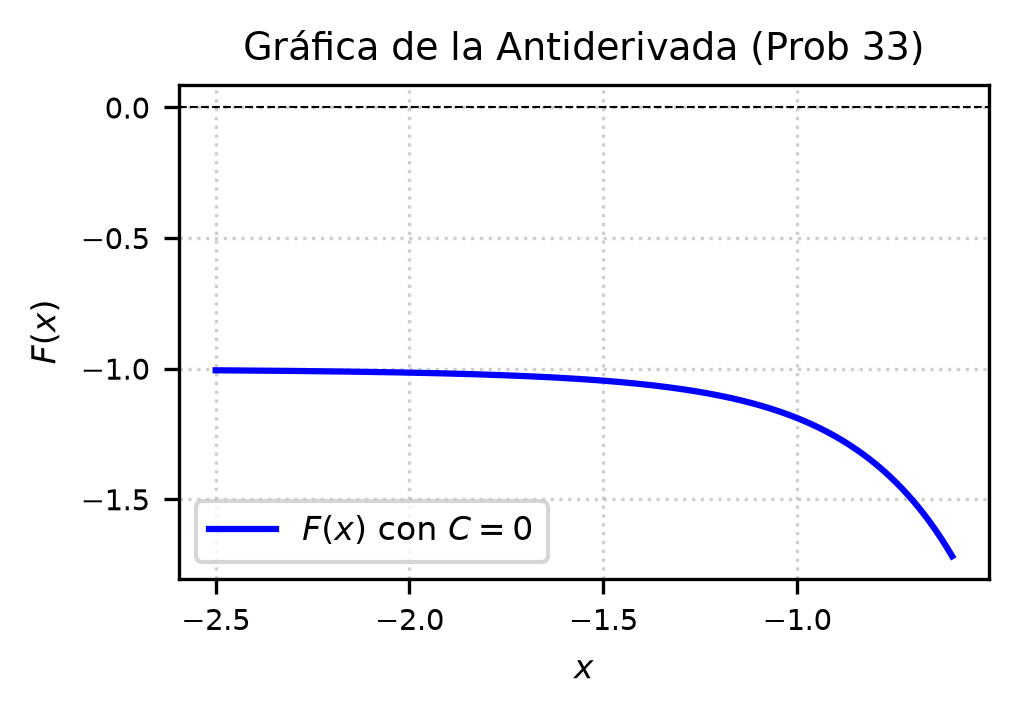
\includegraphics[width=\columnwidth]{semana_05/graficas/SEM05_P33_grafica.png}
	\caption{Representación gráfica de $f(x)$ y su antiderivada $F(x)$ evaluada para la constante de integración $C = 0$ (Problema 33).}
	\label{fig:problema33}
\end{figure}
